\documentclass[12pt,a4paper]{article}
\usepackage[utf8]{vietnam}
\usepackage{amsmath}
\usepackage{amsfonts}
\usepackage{amssymb}
\usepackage{geometry}
\usepackage{graphicx}
\usepackage{float}
\usepackage{booktabs}
\geometry{margin=2.5cm}
\usepackage[hidelinks]{hyperref}

\title{\textbf{Tìm hiểu thuật toán K-Nearest Neighbors (KNN)}}
\author{ye-PHD Lab}
\date{}

\begin{document}

\maketitle
\tableofcontents
\newpage

\section{Thuật toán KNN là gì?}

K-Nearest Neighbors (KNN) là một thuật toán học có giám sát (supervised learning) và phi tham số (non-parametric). Thuật toán hoạt động dựa trên nguyên lý: các điểm dữ liệu tương tự nhau thường nằm gần nhau trong không gian đặc trưng. Từ đó, KNN sử dụng độ gần (proximity) giữa các điểm để thực hiện phân loại hoặc dự đoán giá trị.

\begin{figure}[H]
    \centering
    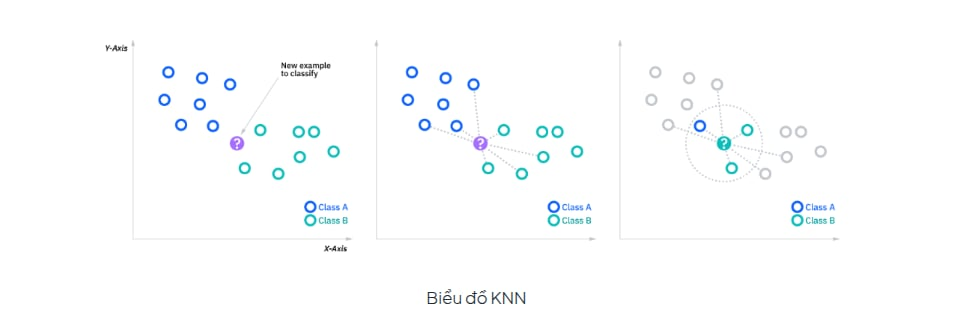
\includegraphics[width=0.85\linewidth]{b4c215ea-de4d-4f7b-946c-eae33dd73f39.jpeg}
    \caption{Minh họa thuật toán KNN (Nguồn: VinBigData)}
\end{figure}

\section{Chuẩn hóa dữ liệu (Feature Scaling)}

Vì KNN tính toán dựa hoàn toàn vào khoảng cách, bất kỳ đặc trưng nào có phạm vi giá trị lớn hơn đều sẽ áp đảo các đặc trưng còn lại. Vì vậy, chuẩn hóa dữ liệu trước khi chạy KNN là bước bắt buộc.

\subsection{Chuẩn hóa Z-score (Standardization)}

Phương pháp này đưa dữ liệu về dạng có giá trị trung bình bằng 0 và độ lệch chuẩn bằng 1. Đặc biệt phù hợp khi dữ liệu tuân theo phân phối chuẩn.

\begin{equation}
    z = \frac{x - \mu}{\sigma}
\end{equation}

Trong đó $x$ là giá trị gốc, $\mu$ là giá trị trung bình, và $\sigma$ là độ lệch chuẩn của đặc trưng.

\subsection{Chuẩn hóa Min-Max (Normalization)}

Phương pháp này nén dữ liệu về một khoảng xác định, thường là $[0, 1]$, trong khi vẫn giữ nguyên mối quan hệ giữa các giá trị gốc.

\begin{equation}
    x' = \frac{x - x_{\min}}{x_{\max} - x_{\min}}
\end{equation}

Lưu ý: phương pháp này nhạy cảm với các điểm ngoại lai (outliers) và thường được dùng với tập dữ liệu nhỏ.

\subsection{Chuẩn hóa độ dài đơn vị (Unit Length Scaling)}

Còn gọi là Scaling to Unit Norm, phương pháp này biến đổi mỗi mẫu dữ liệu sao cho vector kết quả có độ dài (norm) bằng 1, giúp loại bỏ ảnh hưởng về độ lớn và chỉ giữ lại thông tin về hướng.

\begin{equation}
    x_{\text{unit}} = \frac{x}{\sqrt{\sum_{i=1}^{n} x_i^2}}
\end{equation}

Phương pháp này thường được dùng trong các bài toán so sánh độ tương đồng góc (Cosine Similarity).

\section{Các hàm đo khoảng cách trong KNN}

Để xác định "độ gần", thuật toán sử dụng các hàm đo khoảng cách toán học giữa điểm cần dự đoán $x$ và các điểm trong tập huấn luyện $y$.

\subsection{Khoảng cách Euclid (Euclidean Distance)}

Đây là khoảng cách phổ biến nhất — đo đường thẳng nối giữa hai điểm trong không gian $n$ chiều.

\begin{equation}
    d(x, y) = \sqrt{\sum_{i=1}^{n} (x_i - y_i)^2}
\end{equation}

\begin{figure}[H]
    \centering
    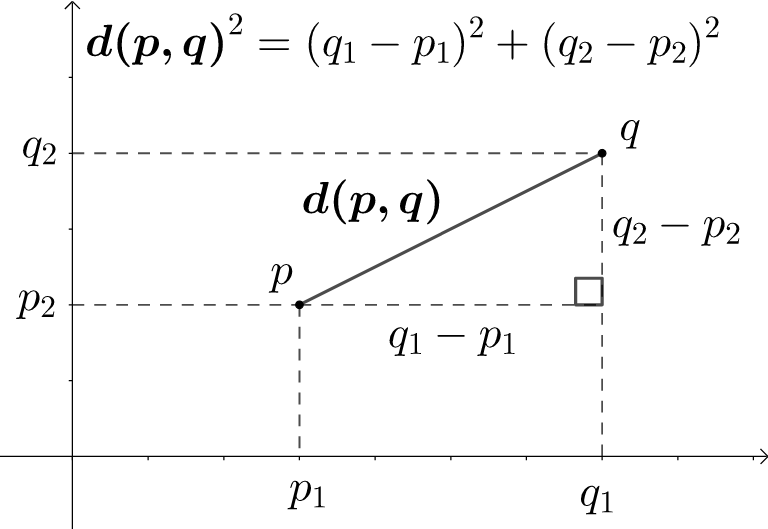
\includegraphics[width=0.45\linewidth]{Euclidean_distance_2d.png}
    \caption{Khoảng cách Euclid (Nguồn: Wikipedia)}
\end{figure}

\subsection{Khoảng cách Manhattan}

Khoảng cách được tính bằng tổng trị tuyệt đối hiệu tọa độ giữa các điểm — phù hợp với không gian lưới.

\begin{equation}
    d(x, y) = \sum_{i=1}^{n} |x_i - y_i|
\end{equation}

\begin{figure}[H]
    \centering
    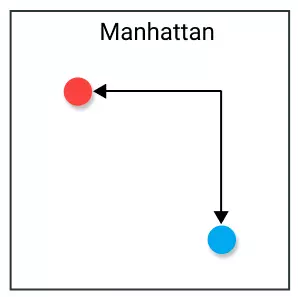
\includegraphics[width=0.45\linewidth]{64f82926-3a2a-4dbc-9bb8-05582c4c0d10.png}
    \caption{Khoảng cách Manhattan (Nguồn: Viblo)}
\end{figure}

\subsection{Khoảng cách Chebyshev}

Khoảng cách Chebyshev chỉ dựa vào chiều có sự chênh lệch lớn nhất giữa hai điểm.

\begin{equation}
    d(x, y) = \max_{i=1}^{n} \left(|x_i - y_i|\right)
\end{equation}

\begin{figure}[H]
    \centering
    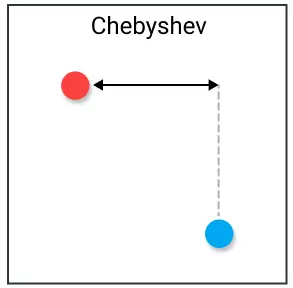
\includegraphics[width=0.45\linewidth]{88defc46-4263-409a-bbcf-54810a1f390a.png}
    \caption{Khoảng cách Chebyshev (Nguồn: Viblo)}
\end{figure}


\section{Tham số $p$ trong khoảng cách Minkowski}

Khoảng cách Minkowski là dạng tổng quát hóa của cả ba khoảng cách trên:

\begin{equation}
    d(x, y) = \left( \sum_{i=1}^{n} |x_i - y_i|^p \right)^{1/p}
\end{equation}

Tham số $p$ quyết định hình dạng vùng lân cận và cách thuật toán "cảm nhận" không gian:
\begin{itemize}
    \item $p = 1$: khoảng cách Manhattan.
    \item $p = 2$: khoảng cách Euclid.
    \item $p \to \infty$: khoảng cách Chebyshev.
\end{itemize}

\subsection{$p = 1$ — Manhattan}

Phù hợp khi các đặc trưng có ý nghĩa độc lập, không thể kết hợp trực tiếp (ví dụ: một trục là Tuổi, một trục là Thu nhập). Ít bị ảnh hưởng bởi ngoại lai hơn so với Euclid.

\subsection{$p = 2$ — Euclid}

Giá trị mặc định trong hầu hết các thư viện Machine Learning. Phản ánh khoảng cách vật lý thực tế trong không gian đa chiều và hoạt động tốt nhất khi dữ liệu đã được chuẩn hóa.

\subsection{$p \to \infty$ — Chebyshev}

Hay còn gọi là khoảng cách bàn cờ (Chessboard distance). Khoảng cách hoàn toàn do chiều có sự chênh lệch lớn nhất quyết định. Thường dùng trong bài toán lập trình quỹ đạo robot hoặc phát hiện bất thường cực đoan trong lưu lượng mạng.

\section{Lựa chọn tham số $K$}

\subsection{Có Validation}

Validation set là tập dữ liệu dùng để tìm ra giá trị $K$ tối ưu. Tỉ lệ tách thường dùng:
\begin{itemize}
    \item $n < 30$: dùng Leave-One-Out — lần lượt dùng từng điểm làm điểm kiểm thử.
    \item $100 \leq n \leq 10{,}000$: tách ngẫu nhiên khoảng 20\% làm Validation set.
    \item $n \geq 100{,}000$: tách khoảng 1--5\%.
\end{itemize}

Sau khi có Validation set, ta cho từng điểm trong đó đi qua tập huấn luyện, tìm $K$ điểm gần nhất, rồi so sánh nhãn dự đoán với nhãn thực tế. Độ chính xác tại mỗi $K$ được tính:

\begin{equation}
    \text{Accuracy} = \frac{\text{Số điểm dự đoán đúng}}{\text{Tổng số điểm Validation}}
\end{equation}

Giá trị khởi điểm thường dùng là $K = \sqrt{N}$ (với $N$ là tổng số mẫu huấn luyện). Đây là điểm cân bằng giữa hai thái cực: $K = 1$ quá nhạy cảm với nhiễu, còn $K = N$ bỏ qua hoàn toàn thông tin khoảng cách và chỉ xét bên nào chiếm đa số.

\subsection{Không có Validation}

Nếu bỏ qua bước Validation, $K$ phải được chọn thủ công vì bản thân KNN không thể tự xác định giá trị này. Trong học máy, $K$ được gọi là siêu tham số (Hyperparameter) — con số do người dùng áp đặt từ bên ngoài trước khi thuật toán chạy.

Các cách chọn $K$ phổ biến khi không có Validation:
\begin{itemize}
    \item Chọn $K = \sqrt{N}$; nếu kết quả là số chẵn thì cộng hoặc trừ 1 để được số lẻ (tránh tình huống hòa phiếu).
    \item Dùng giá trị mặc định $K = 5$ mà nhiều thư viện áp dụng sẵn.
    \item Nếu dữ liệu sạch và phân tách rõ, có thể thử $K = 1$ hoặc $K = 3$.
\end{itemize}

Cách tiếp cận này mang tính kinh nghiệm và không đảm bảo tìm được $K$ tối ưu.


\section{Mô hình Toán học: K-Nearest Neighbors kết hợp Cosine Similarity}
\subsection{Độ tương đồng và Khoảng cách Cosine}

Cho $\mathbf{z}_q \in \mathbb{R}^d$ là vector của mẫu truy vấn và
$\mathbf{z}_i \in \mathbb{R}^d$ là vector của mẫu huấn luyện thứ $i$.
Độ tương đồng Cosine đo lường mức độ cùng hướng giữa hai vector thông
qua góc $\theta$ tạo bởi chúng:

\begin{equation}
    S_C(\mathbf{z}_q, \mathbf{z}_i)
    = \cos\theta
    = \frac{\mathbf{z}_q \cdot \mathbf{z}_i}
           {\|\mathbf{z}_q\|\,\|\mathbf{z}_i\|}
    = \frac{\displaystyle\sum_{j=1}^{d} z_{qj}\,z_{ij}}
           {\displaystyle\sqrt{\sum_{j=1}^{d} z_{qj}^2}
            \sqrt{\sum_{j=1}^{d} z_{ij}^2}}
\end{equation}

Giá trị $S_C \in [-1, 1]$: bằng $1$ khi hai vector hoàn toàn cùng hướng,
bằng $0$ khi vuông góc, và bằng $-1$ khi ngược chiều nhau. Để sử dụng
như một metric khoảng cách (giá trị nhỏ hơn tương ứng với mức độ tương
đồng cao hơn), khoảng cách Cosine được định nghĩa là:

\begin{equation}
    D_C(\mathbf{z}_q, \mathbf{z}_i) = 1 - S_C(\mathbf{z}_q, \mathbf{z}_i)
\end{equation}

Lưu ý rằng $D_C \in [0, 2]$ và bằng $0$ khi và chỉ khi hai vector hoàn
toàn cùng hướng.

\subsection{Xác định láng giềng và Phân loại}

Tập $K$ láng giềng gần nhất của mẫu truy vấn, ký hiệu
$\mathcal{N}_K(\mathbf{z}_q)$, được xác định bằng cách chọn $K$ mẫu
huấn luyện có khoảng cách $D_C$ nhỏ nhất so với $\mathbf{z}_q$.
Nhãn dự đoán $\hat{y}_q$ được quyết định theo nguyên tắc bầu chọn đa số
(majority voting):

\begin{equation}
    \hat{y}_q
    = \underset{c \,\in\, \mathcal{C}}{\mathrm{argmax}}
      \sum_{\mathbf{z}_j \,\in\, \mathcal{N}_K(\mathbf{z}_q)}
      \mathbf{1}\bigl[y_j = c\bigr]
\end{equation}

trong đó $\mathcal{C}$ là tập hợp tất cả các nhãn lớp, và
$\mathbf{1}[\cdot]$ là hàm chỉ thị, nhận giá trị $1$ nếu điều kiện trong
ngoặc được thỏa mãn và $0$ trong trường hợp còn lại. Nói cách khác, mẫu
truy vấn được gán vào lớp xuất hiện nhiều nhất trong $K$ láng giềng của nó.
\section{Hồi quy KNN}

Bên cạnh bài toán phân loại (Classification), KNN còn được dùng cho bài toán hồi quy (Regression) — tức là dự đoán các giá trị liên tục. Thay vì bỏ phiếu, KNN Hồi quy lấy trung bình giá trị của $K$ điểm lân cận:

\begin{equation}
    \hat{y} = \frac{1}{K} \sum_{i \in N_K(x)} y_i
\end{equation}

trong đó $N_K(x)$ là tập $K$ điểm gần nhất với điểm cần dự đoán $x$.

\subsection{So sánh với Linear Regression}

\subsubsection{Khả năng học và tốc độ}

Linear Regression tốn thời gian ở giai đoạn huấn luyện để tối ưu hóa phương trình, nhưng một khi đã có phương trình, việc dự đoán chỉ là một phép tính đơn giản — gần như tức thì.

KNN thì ngược lại: thời gian huấn luyện bằng 0 vì thuật toán chỉ lưu dữ liệu vào bộ nhớ. Tuy nhiên, mỗi lần dự đoán phải tính khoảng cách đến toàn bộ tập huấn luyện. Khi dữ liệu lên đến hàng triệu mẫu, chi phí này trở nên rất đắt đỏ.

\subsubsection{Tuyến tính và phi tuyến}

Linear Regression bị ràng buộc bởi giả định tuyến tính — mô hình luôn khớp một đường thẳng với dữ liệu. Nếu quan hệ thực tế là phi tuyến, độ chính xác sẽ kém.

KNN không bị ràng buộc vào bất kỳ dạng hàm nào, nên đường dự đoán có thể uốn theo mọi cấu trúc của dữ liệu.

\subsubsection{Ngoại suy}

Linear Regression có thể ngoại suy (Extrapolation): kéo dài phương trình ra ngoài miền dữ liệu huấn luyện và vẫn cho ra kết quả có tính nhất quán.

KNN hoàn toàn bất lực trong ngoại suy: nó chỉ có thể nội suy (Interpolation) trong phạm vi dữ liệu đã thấy. Mọi dự đoán đều bị giới hạn bởi giá trị lớn nhất và nhỏ nhất trong tập huấn luyện.

\medskip
\noindent\textbf{Tóm lại:} dữ liệu đơn giản, tuyến tính, cần tốc độ cao $\to$ dùng Linear Regression. Dữ liệu phức tạp, phi tuyến, quy mô nhỏ $\to$ dùng KNN Regression.

\section{Quy trình hoạt động của KNN}

\begin{enumerate}
    \item \textbf{Chọn $K$.} Xác định số lượng láng giềng cần xét. $K$ quá nhỏ dễ gây overfitting; $K$ quá lớn dễ gây underfitting.
    \item \textbf{Tính khoảng cách.} Tính khoảng cách từ điểm cần dự đoán đến tất cả các điểm trong tập huấn luyện (thường dùng Euclid).
    \item \textbf{Tìm $K$ điểm gần nhất.} Sắp xếp khoảng cách tăng dần và chọn $K$ điểm nhỏ nhất.
    \item \textbf{Đưa ra dự đoán.}
    \begin{itemize}
        \item Phân loại: gán nhãn theo nhãn xuất hiện nhiều nhất (Majority Voting).
        \item Hồi quy: lấy trung bình cộng giá trị của $K$ điểm lân cận.
    \end{itemize}
\end{enumerate}

\section{Thử nghiệm}
\subsection{Tính với Euclidean}
Tập dữ liệu gồm 12 mẫu với hai đặc trưng là \textit{SystemCalls} ($X_1$) và \textit{NetworkConnections} ($X_2$), cùng nhãn phân loại \textit{Label}. Thuật toán sử dụng khoảng cách Euclidean ($p = 2$).

\begin{table}[H]
    \centering
    \caption{Tập dữ liệu gốc chưa chuẩn hóa}
    \vspace{0.2cm}
    \renewcommand{\arraystretch}{1.2}
    \begin{tabular}{ccc}
        \toprule
        \textbf{SystemCalls} & \textbf{NetworkConnections} & \textbf{Label} \\
        \midrule
        1 & 1 & 0 \\
        1 & 2 & 0 \\
        2 & 1 & 0 \\
        2 & 2 & 0 \\
        8 & 8 & 1 \\
        8 & 9 & 1 \\
        9 & 8 & 1 \\
        9 & 9 & 1 \\
        5 & 5 & 1 \\
        4 & 7 & 0 \\
        2 & 8 & 0 \\
        7 & 2 & 1 \\
        \bottomrule
    \end{tabular}
\end{table}

Các tham số thống kê tính được từ tập dữ liệu:
\begin{itemize}
    \item $X_1$ (SystemCalls): $\mu_1 = 4.8333$, $\sigma_1 = 3.0777$
    \item $X_2$ (NetworkConnections): $\mu_2 = 5.1667$, $\sigma_2 = 3.1842$
\end{itemize}

\begin{table}[H]
    \centering
    \caption{Chuẩn hóa Z-score cho $X_1$ (SystemCalls)}
    \vspace{0.2cm}
    \renewcommand{\arraystretch}{1.4}
    \begin{tabular}{ccc}
        \toprule
        \textbf{Giá trị gốc ($x_1$)} & \textbf{Phép tính} & \textbf{Z-score} \\
        \midrule
        1 & $(1 - 4.8333) / 3.0777$ & $-1.2455$ \\
        1 & $(1 - 4.8333) / 3.0777$ & $-1.2455$ \\
        2 & $(2 - 4.8333) / 3.0777$ & $-0.9206$ \\
        2 & $(2 - 4.8333) / 3.0777$ & $-0.9206$ \\
        8 & $(8 - 4.8333) / 3.0777$ & $1.0289$ \\
        8 & $(8 - 4.8333) / 3.0777$ & $1.0289$ \\
        9 & $(9 - 4.8333) / 3.0777$ & $1.3538$ \\
        9 & $(9 - 4.8333) / 3.0777$ & $1.3538$ \\
        5 & $(5 - 4.8333) / 3.0777$ & $0.0542$ \\
        4 & $(4 - 4.8333) / 3.0777$ & $-0.2708$ \\
        2 & $(2 - 4.8333) / 3.0777$ & $-0.9206$ \\
        7 & $(7 - 4.8333) / 3.0777$ & $0.7040$ \\
        \bottomrule
    \end{tabular}
\end{table}

\begin{table}[H]
    \centering
    \caption{Chuẩn hóa Z-score cho $X_2$ (NetworkConnections)}
    \vspace{0.2cm}
    \renewcommand{\arraystretch}{1.4}
    \begin{tabular}{ccc}
        \toprule
        \textbf{Giá trị gốc ($x_2$)} & \textbf{Phép tính} & \textbf{Z-score} \\
        \midrule
        1 & $(1 - 5.1667) / 3.1842$ & $-1.3086$ \\
        2 & $(2 - 5.1667) / 3.1842$ & $-0.9945$ \\
        1 & $(1 - 5.1667) / 3.1842$ & $-1.3086$ \\
        2 & $(2 - 5.1667) / 3.1842$ & $-0.9945$ \\
        8 & $(8 - 5.1667) / 3.1842$ & $0.8898$ \\
        9 & $(9 - 5.1667) / 3.1842$ & $1.2039$ \\
        8 & $(8 - 5.1667) / 3.1842$ & $0.8898$ \\
        9 & $(9 - 5.1667) / 3.1842$ & $1.2039$ \\
        5 & $(5 - 5.1667) / 3.1842$ & $-0.0523$ \\
        7 & $(7 - 5.1667) / 3.1842$ & $0.5758$ \\
        8 & $(8 - 5.1667) / 3.1842$ & $0.8898$ \\
        2 & $(2 - 5.1667) / 3.1842$ & $-0.9945$ \\
        \bottomrule
    \end{tabular}
\end{table}

Tập dữ liệu được chia theo phương pháp Hold-out:
\begin{itemize}
    \item \textbf{Tập huấn luyện (Train):} 10 mẫu (mẫu 1, 2, 3, 5, 6, 7, 9, 10, 11, 12).
    \item \textbf{Tập kiểm thử (Test):} Mẫu 4 $(2, 2)$ — Nhãn 0 và Mẫu 8 $(9, 9)$ — Nhãn 1.
\end{itemize}

Ta chọn $K = 3$ và tính khoảng cách Euclidean trong không gian Z-score.

\medskip
\noindent\textbf{Mẫu 4} ($z_4 = [-0.92,\ -0.99]$) — 3 điểm lân cận gần nhất:
\begin{enumerate}
    \item $d(z_4, z_3) = \sqrt{0^2 + 0.31^2} = 0.31 \;\to\;$ Nhãn 0
    \item $d(z_4, z_2) = \sqrt{0.32^2 + 0^2} = 0.32 \;\to\;$ Nhãn 0
    \item $d(z_4, z_1) = \sqrt{0.32^2 + 0.31^2} \approx 0.45 \;\to\;$ Nhãn 0
\end{enumerate}
$\Rightarrow$ Cả $K = 1$ và $K = 3$ đều dự đoán \textbf{Nhãn 0} (chính xác).

\medskip
\noindent\textbf{Mẫu 8} ($z_8 = [1.35,\ 1.20]$) — 3 điểm lân cận gần nhất:
\begin{enumerate}
    \item $d(z_8, z_7) = \sqrt{0^2 + 0.31^2} = 0.31 \;\to\;$ Nhãn 1
    \item $d(z_8, z_6) = \sqrt{0.32^2 + 0^2} = 0.32 \;\to\;$ Nhãn 1
    \item $d(z_8, z_5) = \sqrt{0.32^2 + 0.31^2} \approx 0.45 \;\to\;$ Nhãn 1
\end{enumerate}
$\Rightarrow$ Cả $K = 1$ và $K = 3$ đều dự đoán \textbf{Nhãn 1} (chính xác).

\begin{equation}
    \text{Accuracy}_{K=1} = \frac{2}{2} = 100\%
    \qquad
    \text{Accuracy}_{K=3} = \frac{2}{2} = 100\%
\end{equation}

\begin{table}[H]
    \centering
    \caption{Kết quả độ chính xác trên tập kiểm thử}
    \vspace{0.2cm}
    \renewcommand{\arraystretch}{1.4}
    \begin{tabular}{cccc}
        \toprule
        \textbf{Tham số $K$} & \textbf{Dự đoán đúng} & \textbf{Tổng mẫu} & \textbf{Accuracy} \\
        \midrule
        $K = 1$ & 2 & 2 & 100\% \\
        $K = 3$ & 2 & 2 & 100\% \\
        \bottomrule
    \end{tabular}
\end{table}

\noindent\textbf{Nhận xét:} Khi các điểm kiểm thử nằm sâu trong cụm và xa đường biên quyết định (decision boundary), cả $K = 1$ lẫn $K = 3$ đều cho kết quả tuyệt đối. Điều này cho thấy KNN hoạt động rất ổn định trên các tập dữ liệu có tính phân tách cao.

\textbf{Dự đoán điểm mới: Test$(4, 6)$}

\noindent\textbf{Bước 1 — Chuẩn hóa Z-score:}
\begin{itemize}
    \item $z_1 = \dfrac{4 - 4.8333}{3.0777} \approx -0.2708$
    \item $z_2 = \dfrac{6 - 5.1667}{3.1842} \approx 0.2617$
\end{itemize}
Điểm kiểm thử trong không gian chuẩn hóa: $Z_{\text{test}} = (-0.2708,\ 0.2617)$.

\medskip
\noindent\textbf{Bước 2 — Tính khoảng cách và tìm lân cận:}

\begin{table}[H]
    \centering
    \caption{Khoảng cách từ $Z_{\text{test}}$ đến các điểm lân cận gần nhất}
    \vspace{0.2cm}
    \renewcommand{\arraystretch}{1.4}
    \begin{tabular}{ccccc}
        \toprule
        \textbf{Thứ tự} & \textbf{Mẫu} & \textbf{Tọa độ Z-score} & \textbf{Khoảng cách $d$} & \textbf{Nhãn} \\
        \midrule
        1 & Mẫu 10 $(4, 7)$ & $(-0.2708,\ 0.5758)$ & $0.3141$ & 0 \\
        2 & Mẫu 9 $(5, 5)$  & $(0.0542,\ -0.0523)$ & $0.4519$ & 1 \\
        3 & Mẫu 11 $(2, 8)$ & $(-0.9206,\ 0.8898)$ & $0.9037$ & 0 \\
        \bottomrule
    \end{tabular}
\end{table}

\noindent\textbf{Bước 3 — Kết quả dự đoán:}
\begin{itemize}
    \item $K = 1$: lân cận gần nhất là Mẫu 10 (Nhãn 0) $\to$ dự đoán \textbf{Label 0}.
    \item $K = 3$: ba lân cận gồm \{Mẫu 10, Mẫu 9, Mẫu 11\} với nhãn \{0, 1, 0\}. Theo bỏ phiếu đa số (2/3) $\to$ dự đoán \textbf{Label 0}.
\end{itemize}
\subsection{Tính Độ tương đồng Cosine (Cosine Similarity):}

Sau khi chuẩn hóa ở Bước 1, vector của điểm Test trong không gian
Z-score là:
\begin{equation}
    \mathbf{z}_{\text{test}} = (-0.2708,\ 0.2617)
\end{equation}

Độ dài (norm) của vector này được tính là:
\begin{equation}
    \|\mathbf{z}_{\text{test}}\|
    = \sqrt{(-0.2708)^2 + (0.2617)^2}
    \approx \sqrt{0.0733 + 0.0685}
    \approx 0.3766
\end{equation}

Độ tương đồng Cosine giữa điểm Test và một mẫu huấn luyện
$\mathbf{z}_i$ được tính theo công thức:
\begin{equation}
    S_C(\mathbf{z}_{\text{test}}, \mathbf{z}_i)
    = \frac{\mathbf{z}_{\text{test}} \cdot \mathbf{z}_i}
           {\|\mathbf{z}_{\text{test}}\|\,\|\mathbf{z}_i\|}
    = \frac{z_{\text{test},1}\,z_{i,1} + z_{\text{test},2}\,z_{i,2}}
           {0.3766 \times \|\mathbf{z}_i\|}
\end{equation}

\vspace{0.5cm}
\textbf{Ví dụ 1: Mẫu dòng 10 --- $\mathbf{x}_{10} = (4,\ 7)$, Nhãn 0.}\\
Theo Bảng 2 và Bảng 3, vector chuẩn hóa tương ứng là
$\mathbf{z}_{10} = (-0.2708,\ 0.5758)$.

\begin{itemize}
    \item Độ dài của $\mathbf{z}_{10}$:
    \begin{equation}
        \|\mathbf{z}_{10}\|
        = \sqrt{(-0.2708)^2 + (0.5758)^2}
        \approx \sqrt{0.0733 + 0.3315}
        \approx 0.6362
    \end{equation}

    \item Tích vô hướng:
    \begin{equation}
        \mathbf{z}_{\text{test}} \cdot \mathbf{z}_{10}
        = (-0.2708)(-0.2708) + (0.2617)(0.5758)
        \approx 0.0733 + 0.1507
        = 0.2240
    \end{equation}

    \item Độ tương đồng Cosine:
    \begin{equation}
        S_C(\mathbf{z}_{\text{test}},\, \mathbf{z}_{10})
        = \frac{0.2240}{0.3766 \times 0.6362}
        \approx \frac{0.2240}{0.2396}
        \approx 0.9349
    \end{equation}
\end{itemize}

\textit{Nhận xét: Hai vector gần như cùng hướng ($\theta$ rất nhỏ),
phản ánh mức độ tương đồng lên tới $93.49\%$.}

\vspace{0.5cm}
\textbf{Ví dụ 2: Mẫu dòng 8 --- $\mathbf{x}_8 = (9,\ 9)$, Nhãn 1.}\\
Theo Bảng 2 và Bảng 3, vector chuẩn hóa tương ứng là
$\mathbf{z}_8 = (1.3538,\ 1.2039)$.

\begin{itemize}
    \item Độ dài của $\mathbf{z}_8$:
    \begin{equation}
        \|\mathbf{z}_8\|
        = \sqrt{(1.3538)^2 + (1.2039)^2}
        \approx \sqrt{1.8328 + 1.4494}
        \approx 1.8117
    \end{equation}

    \item Tích vô hướng:
    \begin{equation}
        \mathbf{z}_{\text{test}} \cdot \mathbf{z}_8
        = (-0.2708)(1.3538) + (0.2617)(1.2039)
        \approx -0.3666 + 0.3151
        = -0.0515
    \end{equation}

    \item Độ tương đồng Cosine:
    \begin{equation}
        S_C(\mathbf{z}_{\text{test}},\, \mathbf{z}_8)
        = \frac{-0.0515}{0.3766 \times 1.8117}
        \approx \frac{-0.0515}{0.6823}
        \approx -0.0755
    \end{equation}
\end{itemize}

\textit{Nhận xét: Giá trị $S_C < 0$ cho thấy hai vector lệch nhau quá
$90°$, tức hai mẫu mang đặc trưng đối lập nhau.}

\vspace{0.5cm}
\textbf{Quyết định phân loại (Majority Voting):}\\
Tổng hợp kết quả Cosine Similarity trên toàn bộ tập huấn luyện cho thấy
các láng giềng có độ tương đồng cao nhất đều thuộc Nhãn~0, trong đó mẫu
dòng~10 đạt $S_C = 0.9349$. Áp dụng nguyên tắc bầu chọn đa số, thuật
toán KNN phân loại điểm Test$(4,\ 6)$ vào \textbf{Nhãn~0}.
\end{document}